\documentclass{article}
\usepackage{cmap}
\usepackage[utf8]{inputenc}
\usepackage[english,ukrainian]{babel}
\usepackage{graphicx}
\usepackage{geometry}
\usepackage{listings}
\usepackage{float}
\usepackage{amsmath}
\geometry{
	a4paper,
	left=20mm,
	right=20mm,
	top=15mm,
	bottom=15mm,
}
\lstset{
	language=c,
	tabsize=4,
	keepspaces,
	showstringspaces=false,
}
\graphicspath{ {./pictures} }
\setlength{\parindent}{4em}

\newcommand\subject{Основи електроніки}
\newcommand\lecturer{професор кафедри ПЗ \\ Фечан А.В.}
\newcommand\teacher{доцент кафедри ПЗ \\ Коцун В.І.}
\newcommand\mygroup{ПЗ-22}
\newcommand\lab{2}
\newcommand\theme{Аналіз параметрів кіл змінного струму
	засобами програмного продукту Multisim Live}
\newcommand\purpose{Навчитись аналізувати параметри кіл змінного струму
	засобами програмного продукту Multisim Live}

\begin{document}
\begin{normalsize}
	\begin{titlepage}
		\thispagestyle{empty}
		\begin{center}
			\textbf{МІНІСТЕРСТВО ОСВІТИ І НАУКИ УКРАЇНИ\\
				НАЦІОНАЛЬНИЙ УНІВЕРСИТЕТ "ЛЬВІВСЬКА ПОЛІТЕХНІКА"}
		\end{center}
		\begin{flushright}
			\textbf{ІКНІ}\\
			Кафедра \textbf{ПЗ}
		\end{flushright}
		\vspace{200pt}
		\begin{center}
			\textbf{ЗВІТ}\\
			\vspace{10pt}
			до лабораторної роботи № \lab\\
			\textbf{на тему}: “\textit{\theme}”\\
			\textbf{з дисципліни}: “\subject”
		\end{center}
		\vspace{112pt}
		\begin{flushright}
			
			\textbf{Лектор}:\\
			\lecturer\\
			\vspace{28pt}
			\textbf{Виконав}:\\
			
			студент групи \mygroup\\
			Коваленко Д.М.\\
			\vspace{28pt}
			\textbf{Прийняв}:\\
			
			\teacher\\
			
			\vspace{28pt}
			«\rule{1cm}{0.15mm}» \rule{1.5cm}{0.15mm} 2023 р.\\
			$\sum$ = \rule{1cm}{0.15mm}……………\\
			
		\end{flushright}
		\vspace{\fill}
		\begin{center}
			\textbf{Львів — 2023}
		\end{center}
	\end{titlepage}
		
	\begin{description}
		\item[Тема.] \theme.
		\item[Мета.] \purpose.
	\end{description}

	\section*{Теоретичні відомості}
	
		\section*{Індивідуальне завдання}
	\begin{enumerate}
		\item Згідно отриманого завдання провести розрахунок не розгалуженого кола
		змінного струму .
		\item Побудувати векторну діаграму схеми. Побудову діаграми починаємо з
		відкладання струму (без відображення осі дійсних чисел).
		\item Відтворити схему в середовищі Multisim Live та запустити її симуляцію
		(вважати робочою частотою схеми 1кГц).
		\item Провести аналіз параметрів кола визначити характер схеми та частоту
		резонансу напруг.
		\item Згідно отриманого завдання провести розрахунок розгалуженого кола
		змінного струму.
		\item Відтворити схему в середовищі Multisim Live та запустити її симуляцію
		(вважати робочою частотою схеми 1кГц).
		\item Провести аналіз параметрів кола визначити характер схеми та частоту
		резонансу струмів.
		\item Оформити звіт.
	\end{enumerate}
	
	\begin{figure}[H]
		\centering
		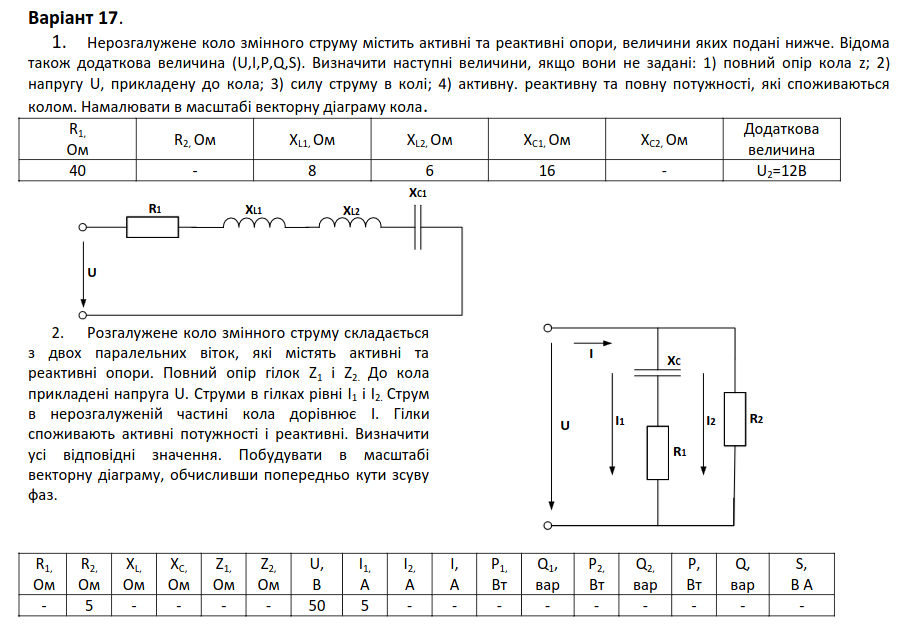
\includegraphics[scale=0.5]{v}
	\end{figure}
	
	\section*{Хід виконання}
	\begin{gather}
		Z=\sqrt{R_{\text{екв}}^2+X_{\text{екв}}^2}\nonumber\\
		Z=\sqrt{R_1^2+(X_{L1}+X_{L2}-X_{C1})^2}\nonumber\\
		Z=\sqrt{40^2+(-2)^2}\approx\text{40 Ом}\nonumber\\
		I=\frac{U_2}{X_{L2}}=\frac{12}{6}=\text{2 А}\nonumber\\
		\phi = \arctg\frac{X_{\text{екв}}}{R_{\text{екв}}}=\arctg\frac{-2}{40}\approx-2.85^\circ\nonumber\\
		U=I\cdot Z=2\cdot40=\text{80 В}\nonumber\\
		P=U\cdot I\cdot\cos\phi=80\cdot2\cdot\cos(-2.85^\circ)\approx\text{160 Вт}\nonumber\\
		Q=U\cdot I\cdot\sin\phi=80\cdot2\cdot\sin(-2.85^\circ)\approx\text{-8 ВАр}\nonumber\\
		S=\sqrt{P^2+Q^2}=\sqrt{160^2+8^2}=\text{224 ВА}\nonumber
	\end{gather}

	\begin{gather}
		U_{R1}=I\cdot R_1=2\cdot40=80\nonumber\\
		U_{XL1}=I\cdot R_{XL1}=2\cdot8=16\nonumber\\
		U_{XL2}=I\cdot R_{XL2}=2\cdot6=12\nonumber\\
		U_{XC1}=I\cdot R_{XC1}=2\cdot16=32\nonumber\\
		\text{(за умовою) f=1000 Гц}\nonumber\\
		\omega=2\pi f=\text{6283 рад/с}\nonumber\\
		L_1=\frac{X_{L1}}{\omega}=\frac{8}{6283}=\text{1.27 мГн}\nonumber\\
		L_2=\frac{X_{L2}}{\omega}=\frac{6}{6283}=\text{0.95 мГн}\nonumber\\
		L=L_1+L_2=\text{2.22 мГн}\nonumber\\
		C_1=\frac{1}{\omega\cdot X_{C1}}=\frac{1}{6283\cdot16}=\text{1 мкФ}\nonumber\\
		C=C_1=\text{1 мкФ}\nonumber
		\omega_p=\sqrt{\frac{1}{L\cdot C}}=21223\nonumber
	\end{gather}

	\section*{Висновки}
	    
\end{normalsize}
\end{document}
